\documentclass[../PhysicsFormulae.tex]{subfiles}
\begin{document}

\subsection{One Way Processes}
The \textit{Entropy Principle} states that in an \underline{irreversible} process, entropy always increases. The reverse of certain processes would have $\Delta S < 0$ if they occurred, violating the entropy principle. Therefore, they do not. \bigskip

There are two approaches to analyzing entropy; one is macroscopic (involving heat and temperature) and the other is microscopic (involving the number theory of particles). 

\subsection{Definining Entropy Change}
For reversible (ideal) processes, entropy change is defined as 
\[ \Delta S = \int_i^f \frac{dQ}{T} \]
and if a process is isothermal, this becomes
\[ \Delta S = \frac{Q}{T} \]

\subsection{Entropy as a State Property}
Taking a differential of the First Law of Thermodynamics, 
\[ dQ = dE_{int} - dW = n C_V dT + p dV \]
and dividing by $T$, 
\[ dS = \frac{dQ}{T} = n C_V \frac{dT}{T} + n R \frac{dV}{V} \] 
Integrating, 
\[ \Delta S = n C_V \ln{\frac{T_f}{T_i}} + n R \ln{\frac{V_f}{V_i}}  \]
Therefore, since temperature and volume are state properties, so is entropy.

\subsection{Entropy Change for Irreversible Processes}
The following method is used to calculate the entropy of an irreversible process: 
\begin{enumerate}
	\item Find a reversible process that connects the same initial and final states. 
	\item Calculate $\Delta S$ for the equivalent reversible process. This entropy change is the same as that of the irreversible one. 
\end{enumerate}
\textbf{Example 1}: Consider a thermally isolated bucket of water. A stone of potential energy $U$ falls into it, causing the temperature of the final system to be greater than before. We would calculate $\Delta S$ by instead imagining that a heater at the bottom of the water increased the temperature by transferring heat $Q = U$ to the water. \bigskip

\textbf{Example 2}: Consider a free expansion of a gas within a thermally isolated container. For the equivalent reversible process, imagine instead that the gas is enclosed by a container with a piston that rises to isothermally increase the volume. 

\subsection{The Second Law of Thermodynamics}
The second law of thermodynamics states that within a closed system, $\Delta S \geq 0$. \bigskip

The $\Delta S = 0$ applies to reversible processes and $\Delta S > 0$ applies to irreversible processes. 

\subsection{Entropy and the Performance of Engines}
A \textit{heat engine} is a device that converts heat to work, with a \textit{working substance} that operates in a cycle. 

\subsubsection{Carnot Engine}
The Carnot Engine is an engine with an Ideal Gas as the working substance and completely reversible processes. 
\begin{figure}
\centering
\begin{minipage}{.5\textwidth}
  \centering
  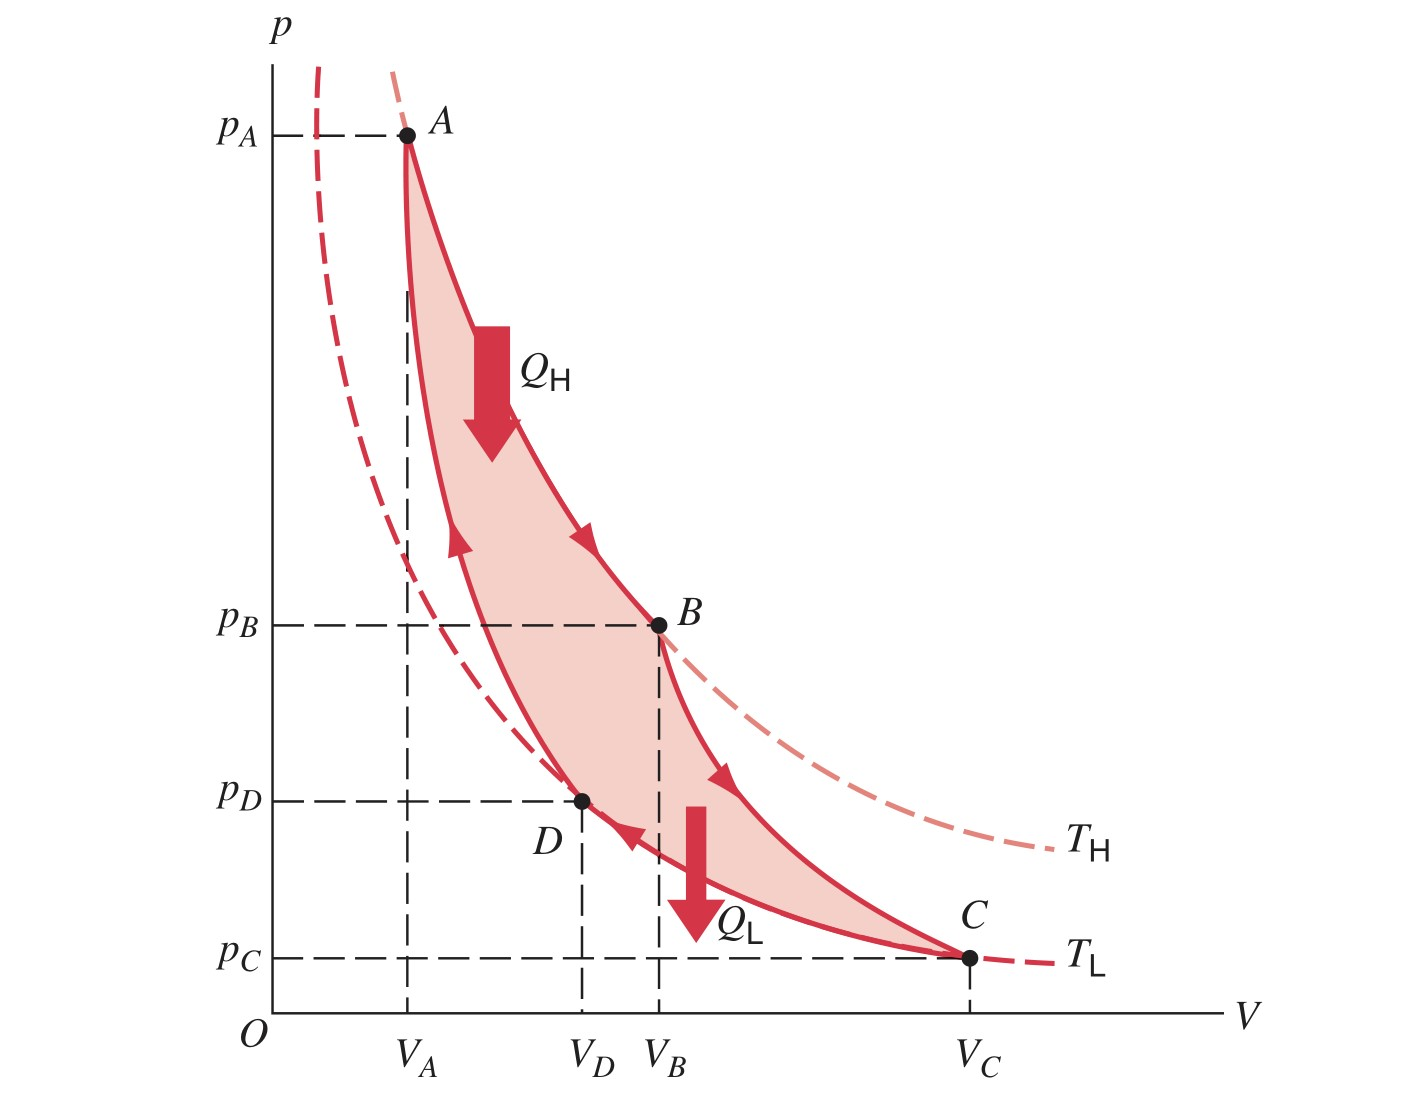
\includegraphics[width=0.8\linewidth]{images/20.carnot_pv.jpg}
  \caption{pV Carnot Plot}
  \label{fig:carnot_pv}
\end{minipage}%
\begin{minipage}{.5\textwidth}
  \centering
  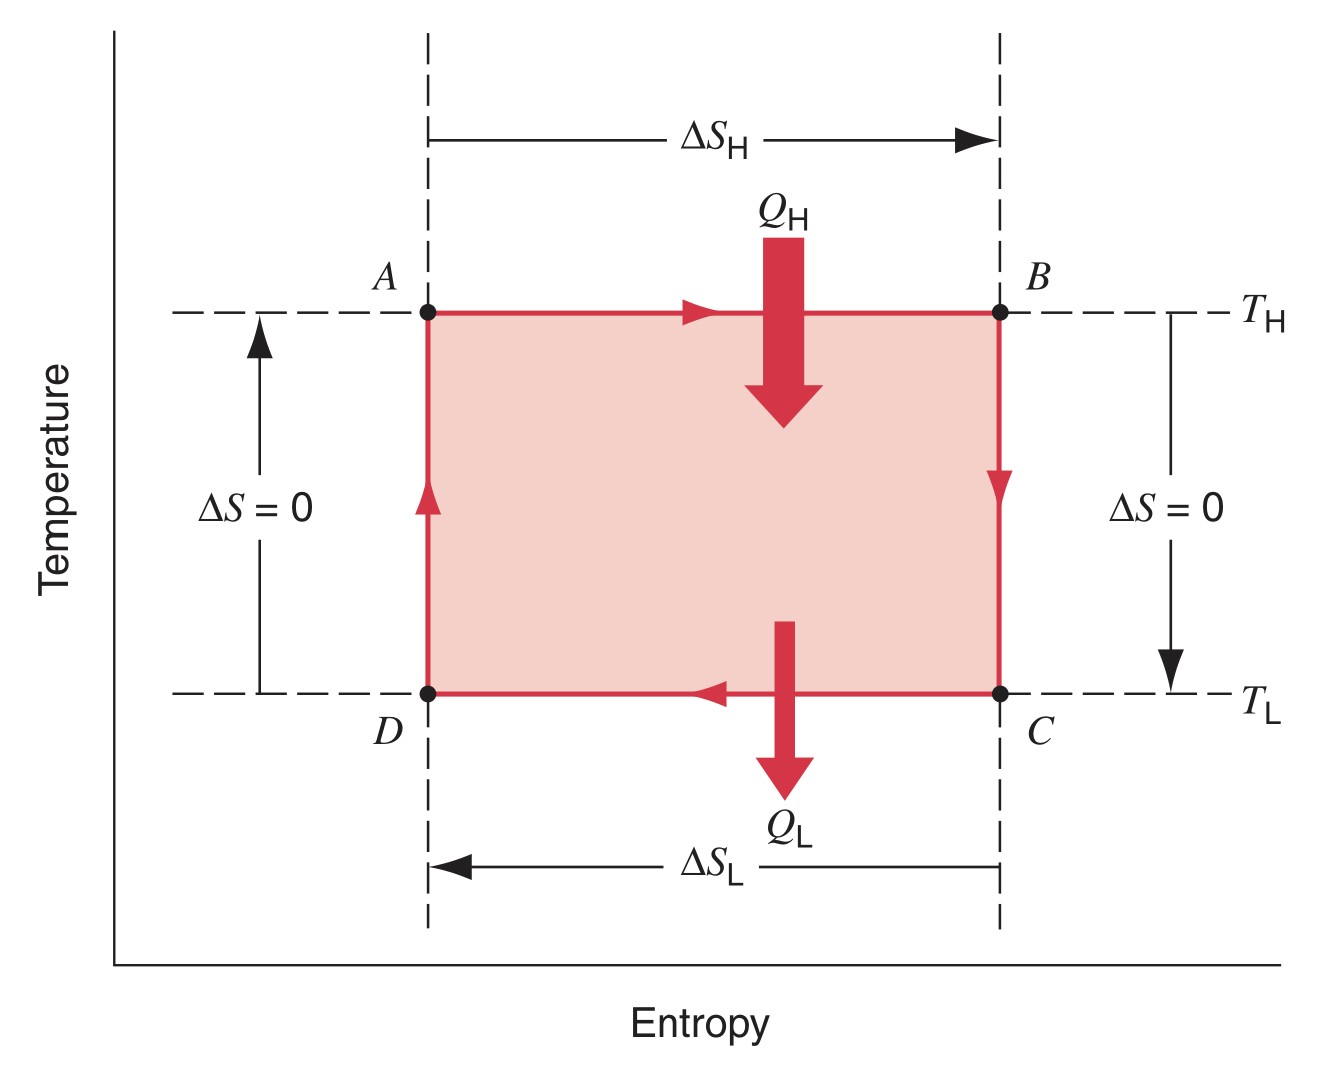
\includegraphics[width=0.8\linewidth]{images/20.carnot_st.jpg}
  \caption{TS Carnot Plot}
  \label{fig:carnot_st}
\end{minipage}
\end{figure}
There are four steps to a Carnot cycle: 
\begin{enumerate}
	\item Isothermal expansion from $V_A$ to $V_B$, as heat is transferred to the container via the hot reservoir at $T_H$. 
	\item Adiabatic expansion from $V_B$ to $V_C$, as the container is placed on an insulating slab. 
	\item Isothermal compression from $V_C$ to $V_D$, as heat is transferred from the container via the cold reservoir at $T_L$. 
	\item Adiabatic compression from $V_D$ to $V_A$, as the container is placed on an insulating slab. 
\end{enumerate}
Consider Figure 5. During expansions AB and BC, the gas is doing positive work \textit{on} the system. But in CD and DA, the gas is doing negative work \textit{on} the system. With engines, it is more convenient to analyze work done by the gas, not on the gas. \bigskip

Consider Figure 6. During AB, the entropy of the gas increases, but during CD, the entropy of the gas decreases. Processes BC and DA are $isentropic$, or constant entropy, processes. 

\subsubsection{Efficiency of a Carnot Engine}
The efficiency is defined as 
\[ \epsilon = \frac{|W|}{|Q_H|} \]
In essence, it is the energy you get relative to the energy you pay for. Since $E_{int}$ of the working substance is a state function, it does not change in one cycle, so $|Q_H| - |Q_L| - |W| = 0$. Therefore, 
\[ \epsilon = \frac{|Q_H| - |Q_L|}{|Q_H|} = 1 - \frac{|Q_L|}{|Q_H|} \]
However, from Figure 6, we can see that 
\[ \Delta S = \frac{|Q_H|}{T_H} - \frac{|Q_L|}{T_L} = 0 \]
Using this result, the efficiency becomes 
\[ \epsilon = 1 - \frac{T_L}{T_H} \]
Necessarily, the efficiency is less than $100\%$ since $T_L < T_H$. Real engines are all less efficient than the Carnot engine. 

\subsubsection{Stirling Engine}
The Stirling Engine involves two two isothermal heat transfers, just like a Carnot engine, but they are instead connected by isometric (constant volume) processes, rather than adiabatic ones. Its ideal efficiency will be lower than that of a Carnot cycle, and real Stirling engines will have lower efficiencies yet. 

\subsection{Entropy and the Performance of Refrigerators}
A \textit{refrigerator} is a device takes in work in order to transfer heat from a lower temperature reservoir to a higher temperature reservoir. 
\begin{itemize}
	\item A household refrigerator uses electrical work to keep its insides cool by transferring heat out. 
	\item An air conditioner keeps a house cool by transferring heat out of the home. 
\end{itemize}
Assuming that the processes are reversible, we have an ideal refrigerator. However, this refrigerator is simply a Carnot engine running backwards, so we call it a Carnot refrigerator. \bigskip

In a refrigerator, the measure of efficiency is the \textit{coefficient of performance} given by 
\[ K = \frac{|Q_L|}{|W|} \]
Like a Carnot engine, we can rewrite it as
\[ K = \frac{|Q_L|}{|Q_H| - |Q_L|} = \frac{T_L}{T_H - T_L} \]
Note that refrigerators are more effective when the temperatures are close together. \bigskip

Can we construct a perfect refrigerator with $W = 0$ and $K \rightarrow \infty$? No, because then entropy change in a cycle would be 
\[ \Delta S = -\frac{|Q|}{T_L} + \frac{|Q|}{T_H} < 0 \]
which violates the second law of thermodynamics. 

\subsection{The Second Law Revisited}
The Second Law of Thermodynamics can be expressed in three ways for closed systems,  
\begin{enumerate}
	\item $\Delta S \geq 0$, or entropy never decreases.
	\item $\epsilon < 100\%$, or there are no perfect engines.
	\item $ K < \infty $, or there are no perfect refrigerators.
\end{enumerate}
While these statements seem different, they are all identical. In deriving the workings of engines and refrigerators, we have seen that statements 2 and 3 result from statement 1. We can also see that statement 2 results from statement 3 by linking up a perfect engine to a Carnot refrigerator; the net effect is to have a perfect refrigerator (a violation of statement 3!). Therefore if statement 3 is true, statement 2 must be too. 

\subsection{A Statistical View of Entropy}
Consider a box, which we will divide into halves to place molecules in. Suppose there are $n$ particles, and we want to split them into a \textit{configuration} of $k$ and $n - k$ portions between the halves. An independent configuration is known as a \textit{microstate}, and the number of ways to arrive at it is the \textit{multiplicity} w, given by
\[ w = \frac{n!}{k!(n - k)!} \]
In essence, we are ``chooosing'' $k$ particles from $n$ total. There are a total of $2^n$ \underline{equally probable} microstates, but note that each configuration is not probable, rather being skewed towards those with high multiplicities. \bigskip

There are \textbf{two important trends} here. 
\begin{enumerate}
	\item The entropy of a system is the \textit{sum} of its subsystems' entropies. 
	\item The probability of a system is the \textit{product} of its subsystems' probabilities. 
\end{enumerate}
Logarithms take products and return sums, so it is logical that they are involved. The actual relationship is 
\[ S = k \ln{w} \]
which is \textit{Boltzmann's entropy equation}, with $k = 1.38 \times 10^{-23}$ being the Boltzmann constant. $w$ is often large enough to result in overflow errors, so we instead use \textit{Stirling's Approximation}, 
\[ \ln{N!} \approx N \ln{N} - N \]

\subsection{Entropy and Disorder}
Entropy is often cast as the amount of disorder in a system, but for this definition to have significance, it must be carefully defined (on a case-to-case basis). One example of this is swirling a cup of tea. 
\begin{itemize}
	\item While swirling, the tea is in uniform angular motion, so there are less possible speeds (and thus few microstates). 
	\item After swirling, the tea is at rest, so there are many more possible speeds due to random motion (and thus many more microstates). 
\end{itemize}
Thus, a swirled cup of tea has more `disorder' and entropy and one at rest. 

\end{document}